\subsection{Hardware}
\begin{frame}
    \frametitle{Server}
    The server will be a Raspberry Pi, with the following specs:

    \begin{tabular}{l l}
        Processor:  & Broadcom 700MHz\\
        RAM:        & 512MB\\
        Graphics:   & VideoCore IV\\
        Hard Drive: & 8GB SD Card\\
        OS:         & Debian Linux (Raspian)\\
    \end{tabular}
\end{frame}

\begin{frame}
    \frametitle{Raspberry Pi Model B}
    \begin{figure}[htb]
        \centering
        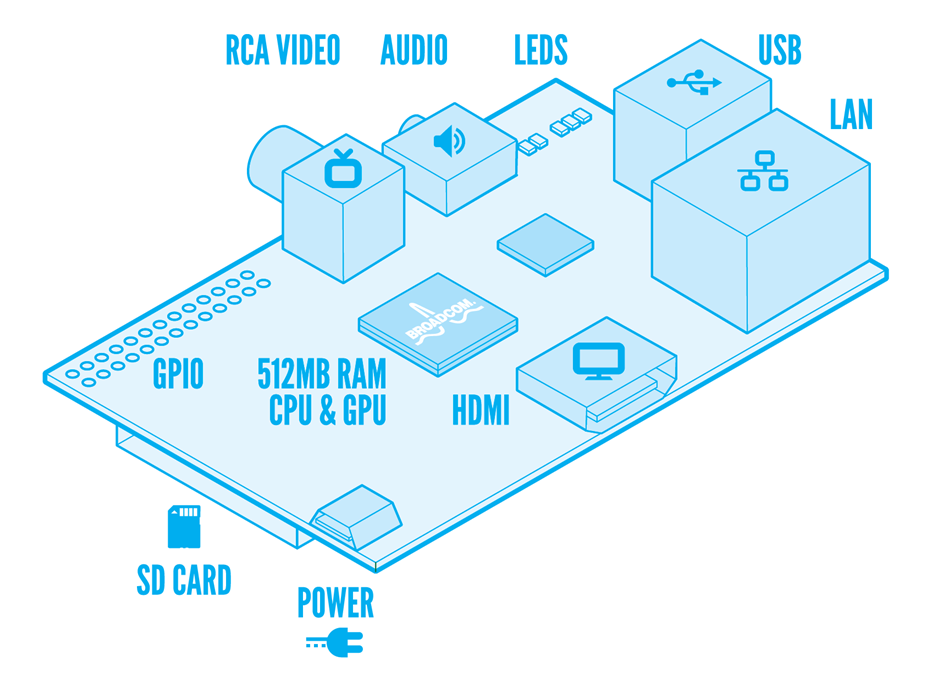
\includegraphics[width=0.8\textwidth]{Images/RaspberryPi.png}
        \caption{Diagram of the Raspberry Pi Model B}
        \label{fig:RaspberryPi}
    \end{figure}
\end{frame}

\subsection{Software}
\begin{frame}
    \frametitle{Server Software}
    \begin{itemize}
        \item {\large Raspian}
        \item {\large Apache2}
        \item {\large PostgreSQL}
    \end{itemize}
\end{frame}

\subsection{Chasis}
\begin{frame}
    \frametitle{Chasis Mock-up}
    \begin{figure}[htb]
        \centering
        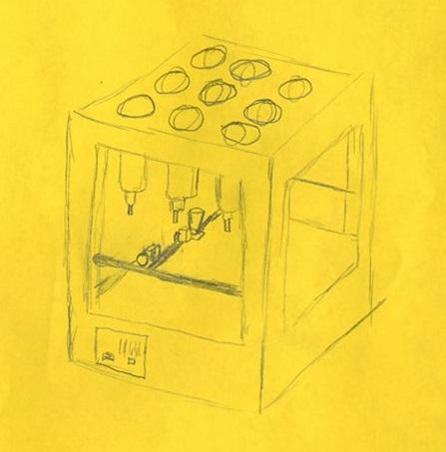
\includegraphics[width=0.6\textheight]{Images/ChasisMockup.png}
        \caption{Diagram of the Chasis}
        \label{fig:ChasisMockUp}
    \end{figure}
\end{frame}

